\documentclass[10pt,a4paper,oneside]{article}
\usepackage[utf8]{inputenc}
\usepackage{amsmath}
\usepackage{draftwatermark} % 设置水印
\SetWatermarkText{DNV Group} % 水印内容
\usepackage{amsfonts}
\usepackage{amssymb}
\usepackage{graphicx}
\usepackage{breqn}
\usepackage{tikz} % system block diagram
\usepackage{textcomp}
\usetikzlibrary{shapes,arrows} % system block diagram
\usepackage{booktabs}
\usepackage[framed,numbered,autolinebreaks,useliterate]{mcode} % matlab code block
\author{Yangang Cao}
\date{February 18, 2019}
\newcommand{\degree}{^\circ}
\tikzset{
	delay/.style    = {draw, thick, rectangle, minimum height = 3em,
		minimum width = 3em},
	sum/.style      = {draw, circle, node distance = 2cm}, 
	prod/.style     = {draw, circle, node distance = 2cm},
	input/.style    = {coordinate}, % Input
	output/.style  = {coordinate} % Output
}
% Defining string as labels of certain blocks.
\newcommand{\product}{$\displaystyle \times$}
\newcommand{\delay}{\large$z^{-1}$}
\begin{document}

\title{First-Order Low/High-Frequency Shelving Filter Design}
\maketitle 
In contrast to low/highpass and bandpass/reject filters, which attenuate the audio spectrum above or below a cut-off frequency, equalizers shape the audio spectrum by enhancing certain frequency bands while others remain unaffected. They are typically built by a series connection of first-and second-order shelving and peak filters, which are controlled independently.\\

Shelving filters boost or cut the low- or high-frequency bands with the parameters cut-off frequency $f_c$ and gain $G$. Similar to the first-order lowpass/highpass filters design, first-order low/high frequency shelving filters can be constructed based on a first-order allpass, yielding the transfer function
\[
H(z) = 1 + \frac{H_0}{2}[1 \pm A(z)]\quad(LF/HF+/-)
\]
with the first-order allpass
\[
A(z) = \frac{z^{-1} + c_{B/C}}{1 + c_{B/C}z^{-1}}.
\]

The block diagram in following figure shows a first-order low/high-frequency shelving filter.
\begin{center}
	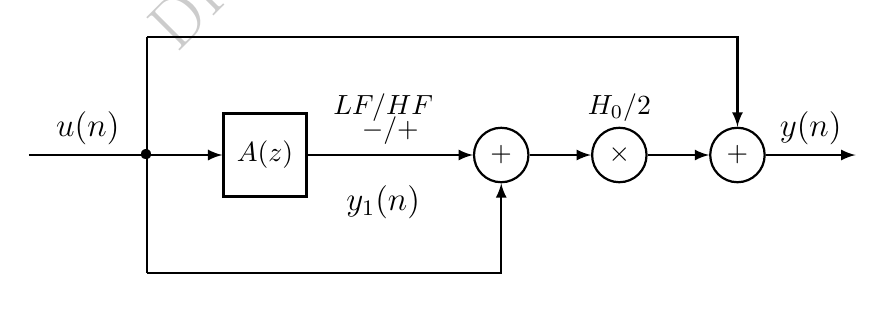
\begin{tikzpicture}[auto, thick, node distance=0.6cm, >=latex, scale = 0.75]
	\draw
	node at (2,0)[delay] (d1) {$A(z)$}
	node at (6,0)[sum] (s1) {$+$}
	node at (8,0)[prod](p1){$\times$} node[above of = p1]{$H_0/2$}
	node at (10,0)[sum](s2){$+$}
	node at (4,0)(n1){}
	node[above of = n1]{$LF/HF$} node[below of =n1]{\large$y_1(n)$}
	;
	
	\draw[-](-2,0) -- node {\large$u(n)$}(0,0);
	\draw[->](0,0) -- node {} (d1);
	\draw[->](d1) -- node {$-/+$} (s1);
	\draw[-](0,0) -- node {} (0,-2);
	\draw[->](0,-2) -| node {} (s1);
	\draw[->](s1) -- node {} (p1);
	\draw[->](p1) -- node {} (s2);
	\draw[->](s2) -- node {\large$y(n)$} (12,0);
	\draw[-](0,0) -- node {} (0,2);
	\draw[->](0,2) -| node {} (s2);
	
	\draw
	node at (0,0) {\textbullet};
	\end{tikzpicture}
\end{center}

The difference equations of first-order low shelving filter are
\[
x(n) = u(n) - c_{B/C}x(n-1)
\]
\[
y_1(n) = c_{B/C}x(n) + x(n-1)
\]
\[
y(n) = \frac{H_0}{2}[u(n) - y_1(n)] + u(n),
\]
and corresponding state and output equations are
\[
x(n) = -c_{B/C}x(n-1) + u(n)
\]
\[
y(n) = \frac{H_0}{2}(1-c^2)x(n-1) + [\frac{H_0}{2}(1+c)+1]u(n).
\]

The gain $G$ in dB for low/high frequencies can be adjusted by the parameter
\[
H_0 = V_0 - 1\quad \mbox{with} \quad V_0 = 10^{G/20}.
\]
The cut-off frenquency parameters, $c_B$ for boost and $c_C$ for cut, for a first-order low-frequency shelving filter can be calculated as
\[
c_B = \frac{\tan(\pi f_c/f_S) - 1}{\tan(\pi f_c/f_S) + 1}
\]
\[
c_C = \frac{\tan(\pi f_c/f_S) - V_0}{\tan(\pi f_c/f_S) + V_0}.
\]

An implementation of first-order low-frenquency shelving filter is given in following {\bfseries Matlab} code.
\begin{lstlisting}
function y = lowshelvingunit(audio, para)
% Applies a low-frequency shelving filter to the input signal.
% para(1) is the normalized cut-off frequency in (0,1), i.e. 2*fc/fs
% para(2) is the gain in dB
V0 = 10^(para(2)/20); H0 = V0 - 1;
if para(2) >= 0
	c = (tan(pi*para(1)/2)-1) / (tan(pi*para(1)/2)+1);     % boost
else
	c = (tan(pi*para(1)/2)-V0) / (tan(pi*para(1)/2)+V0);   % cut
end
x = 0;
x_1 = 0;
for n=1:length(audio)
	x_1 = -c * x + audio(n);
	y(n) = H0 / 2 * (1-c^2) * x + [H0 / 2 * (1+c) + 1] * audio(n);
	x = x_1;
end
\end{lstlisting}

The difference equations of first-order high-shelving filter are
\[
x(n) = u(n) - c_{B/C}x(n-1)
\]
\[
y_1(n) = c_{B/C}x(n) + x(n-1)
\]
\[
y(n) = \frac{H_0}{2}[u(n) + y_1(n)] + u(n),
\]
and corresponding state and output equations are
\[
x(n) = -c_{B/C}x(n-1) + u(n)
\]
\[
y(n) = \frac{H_0}{2}(c^2-1)x(n-1) + [\frac{H_0}{2}(1-c)+1]u(n).
\]

The gain $G$ in dB for low/high frequencies can be adjusted by the parameter
\[
H_0 = V_0 - 1\quad \mbox{with} \quad V_0 = 10^{G/20}.
\]
The cut-off frenquency parameters, $c_B$ for boost and $c_C$ for cut, for a first-order high-frequency shelving filter can be calculated as
\[
c_B = \frac{\tan(\pi f_c/f_S) - 1}{\tan(\pi f_c/f_S) + 1}
\]
\[
c_C = \frac{V_0\tan(\pi f_c/f_S) - 1}{V_0\tan(\pi f_c/f_S) + 1}.
\]

An implementation of first-order high-frenquency shelving filter is given in following {\bfseries Matlab} code.
\begin{lstlisting}
function y = highshelvingunit(audio, para)
% Applies a high-frequency shelving filter to the input signal.
% para(1) is the normalized cut-off frequency in (0,1), i.e. 2*fc/fs
% para(2) is the gain in dB
V0 = 10^(para(2)/20); H0 = V0 - 1;
if para(2) >= 0
c = (tan(pi*para(1)/2)-1) / (tan(pi*para(1)/2)+1);     % boost
else
c = (tan(pi*para(1)/2)-V0) / (tan(pi*para(1)/2)+V0);   % cut
end
x = 0;
x_1 = 0;
for n=1:length(audio)
	x_1 = -c * x + audio(n);
	y(n) = H0/2 * (c^2-1) * x + (H0/2 * (1-c) + 1) * audio(n);
	x = x_1;
end
\end{lstlisting}
\end{document}
